\documentclass{standalone}
\usepackage[T1]{fontenc}
\usepackage[latin2]{inputenc}
\usepackage[english]{babel}
\usepackage{tikz}
\usetikzlibrary{calc,through,backgrounds,positioning,fit}
\usetikzlibrary{shapes,arrows,shadows}
\tikzstyle{stt}=[shape=circle, draw, minimum height=6mm]

\begin{document}

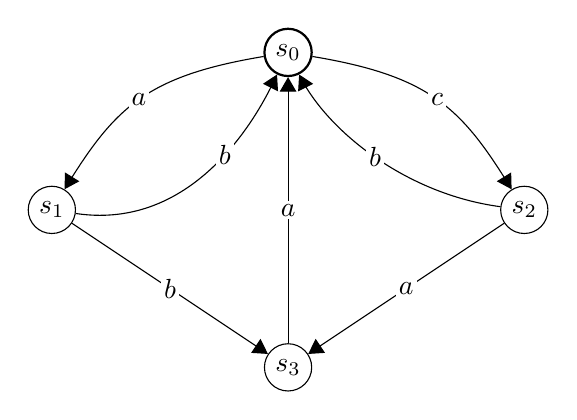
\begin{tikzpicture}[scale=1,inner sep=0.4mm]

\node (s0) [stt,thick] at (0,2) {$s_0$};
\node (s1) [stt] at (-3,0) {$s_1$};
\node (s2) [stt] at (3,0) {$s_2$};
\node (s3) [stt] at (0,-2) {$s_3$};
 
\draw[-triangle 60] (s0) .. node [fill=white] {$c$} controls (1.8,1.7) and (2.2,1.3) .. (s2);
\draw[-triangle 60] (s2) .. node [fill=white] {$b$} controls (1.5,0.2) and (0.5,1) .. (s0);

\draw[-triangle 60] (s0) .. node [fill=white] {$a$} controls (-1.8,1.7) and (-2.2,1.3)  .. (s1);
\draw[-triangle 60] (s1) .. node [fill=white] {$b$} controls (-1,-0.3) and (-0.2,1.6)  .. (s0);

\draw[-triangle 60] (s2) -- node [fill=white] {$a$} (s3);
\draw[-triangle 60] (s1) -- node [fill=white] {$b$} (s3);
\draw[-triangle 60] (s3) -- node [fill=white] {$a$} (s0);
 
\end{tikzpicture}

\end{document}